\documentclass{article}
\usepackage[UTF8]{ctex}
\usepackage[a4paper,margin=2.5cm]{geometry}
\usepackage{graphicx}
\usepackage{booktabs}
\usepackage{amsmath,amssymb}
\usepackage{hyperref}
\usepackage{listings}
\usepackage{xcolor}
\usepackage{subcaption}
\usepackage{natbib}
\usepackage{enumitem}

\bibliographystyle{plainnat}

\lstset{
  basicstyle=\small\ttfamily,
  keywordstyle=\color{blue},
  commentstyle=\color{gray},
  stringstyle=\color{orange},
  numbers=left,
  numberstyle=\tiny\color{gray},
  frame=single,
  breaklines=true,
  language=Python,
}

\title{Deep Reinforcement Learning for Beer Game Supply Chain Ordering}
\author{}
\date{\today}

\begin{document}
\maketitle

\begin{abstract}
  啤酒游戏（Beer Game）是供应链管理与多智能体强化学习中的经典实验平台。本研究基于课程提供的三阶串行供应链环境，针对单企业利润优化任务，系统复现并改进了 DQN、PPO 与 SAC 三类深度强化学习算法。研究重点在于：在保持环境机制（$t+1$ 到货延迟、局部 3 维观测）不变的前提下，通过算法稳定化技巧（GAE、reward scaling、KL early stopping、best-checkpoint 恢复）以及 reward shaping / centralized critic 等算法扩展，提升 PPO 在该离散订货任务上的稳定性与最终性能。实验结果表明，Dueling Double DQN 仍是当前最稳健的基线（3-seed 平均奖励 804.46），而改进后的 PPO 在多数 seed 上达到 790--830 区间，但尚未在所有 seed 上稳定超过 DQN。本报告记录了研究方案、核心实现、实验结果与未来方向。
\end{abstract}

\section{引言}

啤酒游戏模拟了由零售商、批发商、制造商等组成的多阶串行供应链。每阶企业仅掌握局部信息（自身库存、到货、需求），需要在需求波动、订货延迟和库存成本之间做出订货决策。由于牛鞭效应（bullwhip effect），局部理性决策往往导致系统整体低效，是研究多智能体协作与分散决策的典型场景。

本课题的任务目标为：选择链上一个企业，通过深度强化学习优化其长期累积利润，其余企业视为环境的一部分。本研究围绕以下问题展开：
\begin{enumerate}[label=(\arabic*)]
  \item 在课程基线 DQN 上，Double DQN、Dueling 网络等改进能否带来稳定提升？
  \item 策略梯度类方法（PPO）在该离散、短 episode、随机背景策略的任务上表现如何？
  \item 通过 reward shaping、centralized critic、best checkpoint 等算法扩展，能否让 PPO 稳定超过基于值函数的方法？
\end{enumerate}

\section{环境设定}

\subsection{供应链结构}

实验环境包含 3 个串行企业：
\begin{equation}
  \text{外部顾客} \rightarrow \text{企业 0} \rightarrow \text{企业 1} \rightarrow \text{企业 2}.
\end{equation}

本研究固定优化企业 1（中间商），其余企业由背景策略控制。每个企业的局部观测为 3 维向量：
\begin{equation}
  s_t = \bigl[\text{上一期订货量},\ \text{上一期满足需求量},\ \text{当前库存}\bigr].
\end{equation}

动作空间为离散集合 $a_t \in \{0,1,\dots,20\}$，表示当前向上游的订货量。

\subsection{$t+1$ 到货机制}

环境采用课程原始设定：$t$ 时刻发出的订单不会立即进入库存，而是在 $t+1$ 时刻作为在途货物到达。该延迟加剧了需求信息扭曲，是牛鞭效应的主要来源之一。

\subsection{奖励函数}

单步奖励按当期利润计算：
\begin{equation}
  r_t = p_i \cdot d_i^{\text{sat}} - p_{i+1} \cdot o_i - h \cdot I_i - c \cdot \max(D_i - d_i^{\text{sat}}, 0),
\end{equation}
其中 $p_i$ 为售价，$p_{i+1}$ 为采购价，$h$ 为单位库存持有成本，$c$ 为单位缺货惩罚，$I_i$ 为库存，$D_i$ 为下游需求，$d_i^{\text{sat}}$ 为实际满足的需求量。对于最上游企业，采购成本项为 0。

\section{算法设计}

\subsection{DQN 系列基线}

基于课程提供的 DQN，本研究实现了以下消融：
\begin{itemize}[leftmargin=2em]
  \item \textbf{DQN}：标准深度 Q 网络 \citep{mnih2015human}。
  \item \textbf{Double DQN}：使用在线网络选动作、目标网络估值，缓解 Q 值高估 \citep{van2016deep}。
  \item \textbf{Dueling DQN}：将 Q 函数分解为状态值 $V(s)$ 与优势函数 $A(s,a)$ 之和 \citep{wang2016dueling}。
  \item \textbf{Dueling Double DQN}：同时融合 Double 目标与 Dueling 结构。
\end{itemize}

所有 DQN 变体共享超参数：隐藏层 64--64、经验池 10000、批量 64、目标网络软更新 $\tau=0.001$、$\epsilon$ 从 1.0 衰减至 0.05。

\subsection{PPO 实现与改进}

\subsubsection{基础 PPO}

PPO 采用离散动作 Actor-Critic 架构 \citep{schulman2017proximal}，目标函数为 Clipped Surrogate Objective：
\begin{equation}
  L^{\text{CLIP}}(\theta) = \hat{\mathbb{E}}_t\left[\min\left(r_t(\theta)\hat{A}_t, \text{clip}(r_t(\theta),1-\epsilon,1+\epsilon)\hat{A}_t\right)\right],
\end{equation}
其中 $r_t(\theta)=\pi_\theta(a_t|s_t)/\pi_{\theta_{\text{old}}}(a_t|s_t)$，优势函数 $\hat{A}_t$ 通过 GAE 计算 \citep{schulman2015high}：
\begin{equation}
  \hat{A}_t = \delta_t + (\gamma\lambda)\delta_{t+1} + \cdots + (\gamma\lambda)^{T-t}\delta_T.
\end{equation}

\subsubsection{稳定化技巧}

为了提升 PPO 在小样本、离散动作任务上的稳定性，本研究实现了以下改进：
\begin{enumerate}[label=(\arabic*)]
  \item \textbf{Reward scaling}：将原始奖励乘以 0.001，使 PPO 的 value loss 与 policy loss 量级匹配。
  \item \textbf{Clipped value loss}：对 value function 的更新也使用 clipping，避免 value 网络剧烈变化。
  \item \textbf{Gradient clipping}：限制梯度范数最大为 0.5。
  \item \textbf{KL early stopping}：每次 update epoch 后估计 $D_{\text{KL}}(\pi_{\text{old}}\|\pi_{\text{new}})$，若超过 0.015 则提前终止该轮更新。
  \item \textbf{Learning rate / entropy decay}：训练过程中线性衰减学习率与熵正则系数。
  \item \textbf{Best checkpoint}：每 50 个 episode 在固定 20 个 episode 上评估当前策略，保存并恢复最优检查点。
\end{enumerate}

\subsubsection{算法扩展}

在基础 PPO 之上，还尝试以下扩展：
\begin{itemize}[leftmargin=2em]
  \item \textbf{Centralized critic}：Critic 观测全局状态（3 个企业的局部观测拼接），Actor 仍使用局部观测。
  \item \textbf{Reward shaping}：包括 SRDQN 风格的反馈奖励（奖励代理其他企业的平均利润）、外部性惩罚（库存与缺货成本）、动作平滑惩罚等 \citep{ Chavez2020}。
  \item \textbf{EMA evaluation model}：维护策略网络的指数移动平均副本，用于更稳定的评估。
\end{itemize}

\subsection{SAC 基线}

本研究还实现了离散动作 SAC \citep{haarnoja2018soft} 作为补充对比，采用 twin Q 网络与自动熵调节，但在本任务上表现不稳定（详见实验结果）。

\section{实验设置}

\subsection{超参数与训练流程}

主要实验在 3 个随机种子 $[42,123,456]$ 上重复，每个 seed 训练后使用 20 个 episode 评估。PPO 训练 1000 个 episode，DQN 系列训练 300 个 episode。评估时背景策略固定为 random。

PPO 关键超参数如表 \ref{tab:ppo-hparams} 所示。

\begin{table}[htbp]
  \centering
  \caption{PPO 关键超参数}
  \label{tab:ppo-hparams}
  \begin{tabular}{lc}
    \toprule
    超参数 & 默认值 \\
    \midrule
    hidden size & 256 \\
    batch size & 256 \\
    learning rate & $1\times10^{-4}$ \\
    rollout episodes & 4 \\
    update epochs & 20 \\
    clip $\epsilon$ & 0.2 \\
    value coef & 0.5 \\
    entropy coef & 0.05 \\
    target KL & 0.015 \\
    reward scale & 0.001 \\
    max grad norm & 0.5 \\
    GAE $\lambda$ & 0.95 \\
    \bottomrule
  \end{tabular}
\end{table}

\subsection{评估指标}

采用 3-seed 平均奖励（mean reward）作为主要指标，并报告每个 seed 的均值以及跨 seed 标准差，以衡量算法稳定性。

\section{实验结果}

\subsection{算法消融结果}

表 \ref{tab:main-results} 给出了所有基线与改进算法在 3-seed 上的评估结果。

\begin{table}[htbp]
  \centering
  \caption{各算法 3-seed 评估结果（每个 seed 20 episode）}
  \label{tab:main-results}
  \begin{tabular}{lccc}
    \toprule
    方法 & 平均 reward & 标准差 & seed 均值 \\
    \midrule
    random & $-3435.22$ & 2511.29 & $-2659.18$ / $-4013.85$ / $-3632.62$ \\
    base\_stock & $-3885.23$ & 824.78 & $-3979.18$ / $-3787.88$ / $-3888.65$ \\
    DQN & 760.93 & 109.97 & 789.95 / 744.67 / 748.17 \\
    Double DQN & 797.19 & 117.85 & 813.00 / 777.22 / 801.35 \\
    Dueling DQN & 781.23 & 126.05 & 792.53 / 762.03 / 789.15 \\
    Dueling Double DQN & \textbf{804.46} & 114.58 & 838.55 / 787.10 / 787.72 \\
    PPO（改进后） & 779.59 & 123.68 & 753.50 / 784.72 / 800.55 \\
    SAC & $-7305.86$ & 6426.45 & $-11431.58$ / $-11120.33$ / 634.33 \\
    \bottomrule
  \end{tabular}
\end{table}

\begin{figure}[htbp]
  \centering
  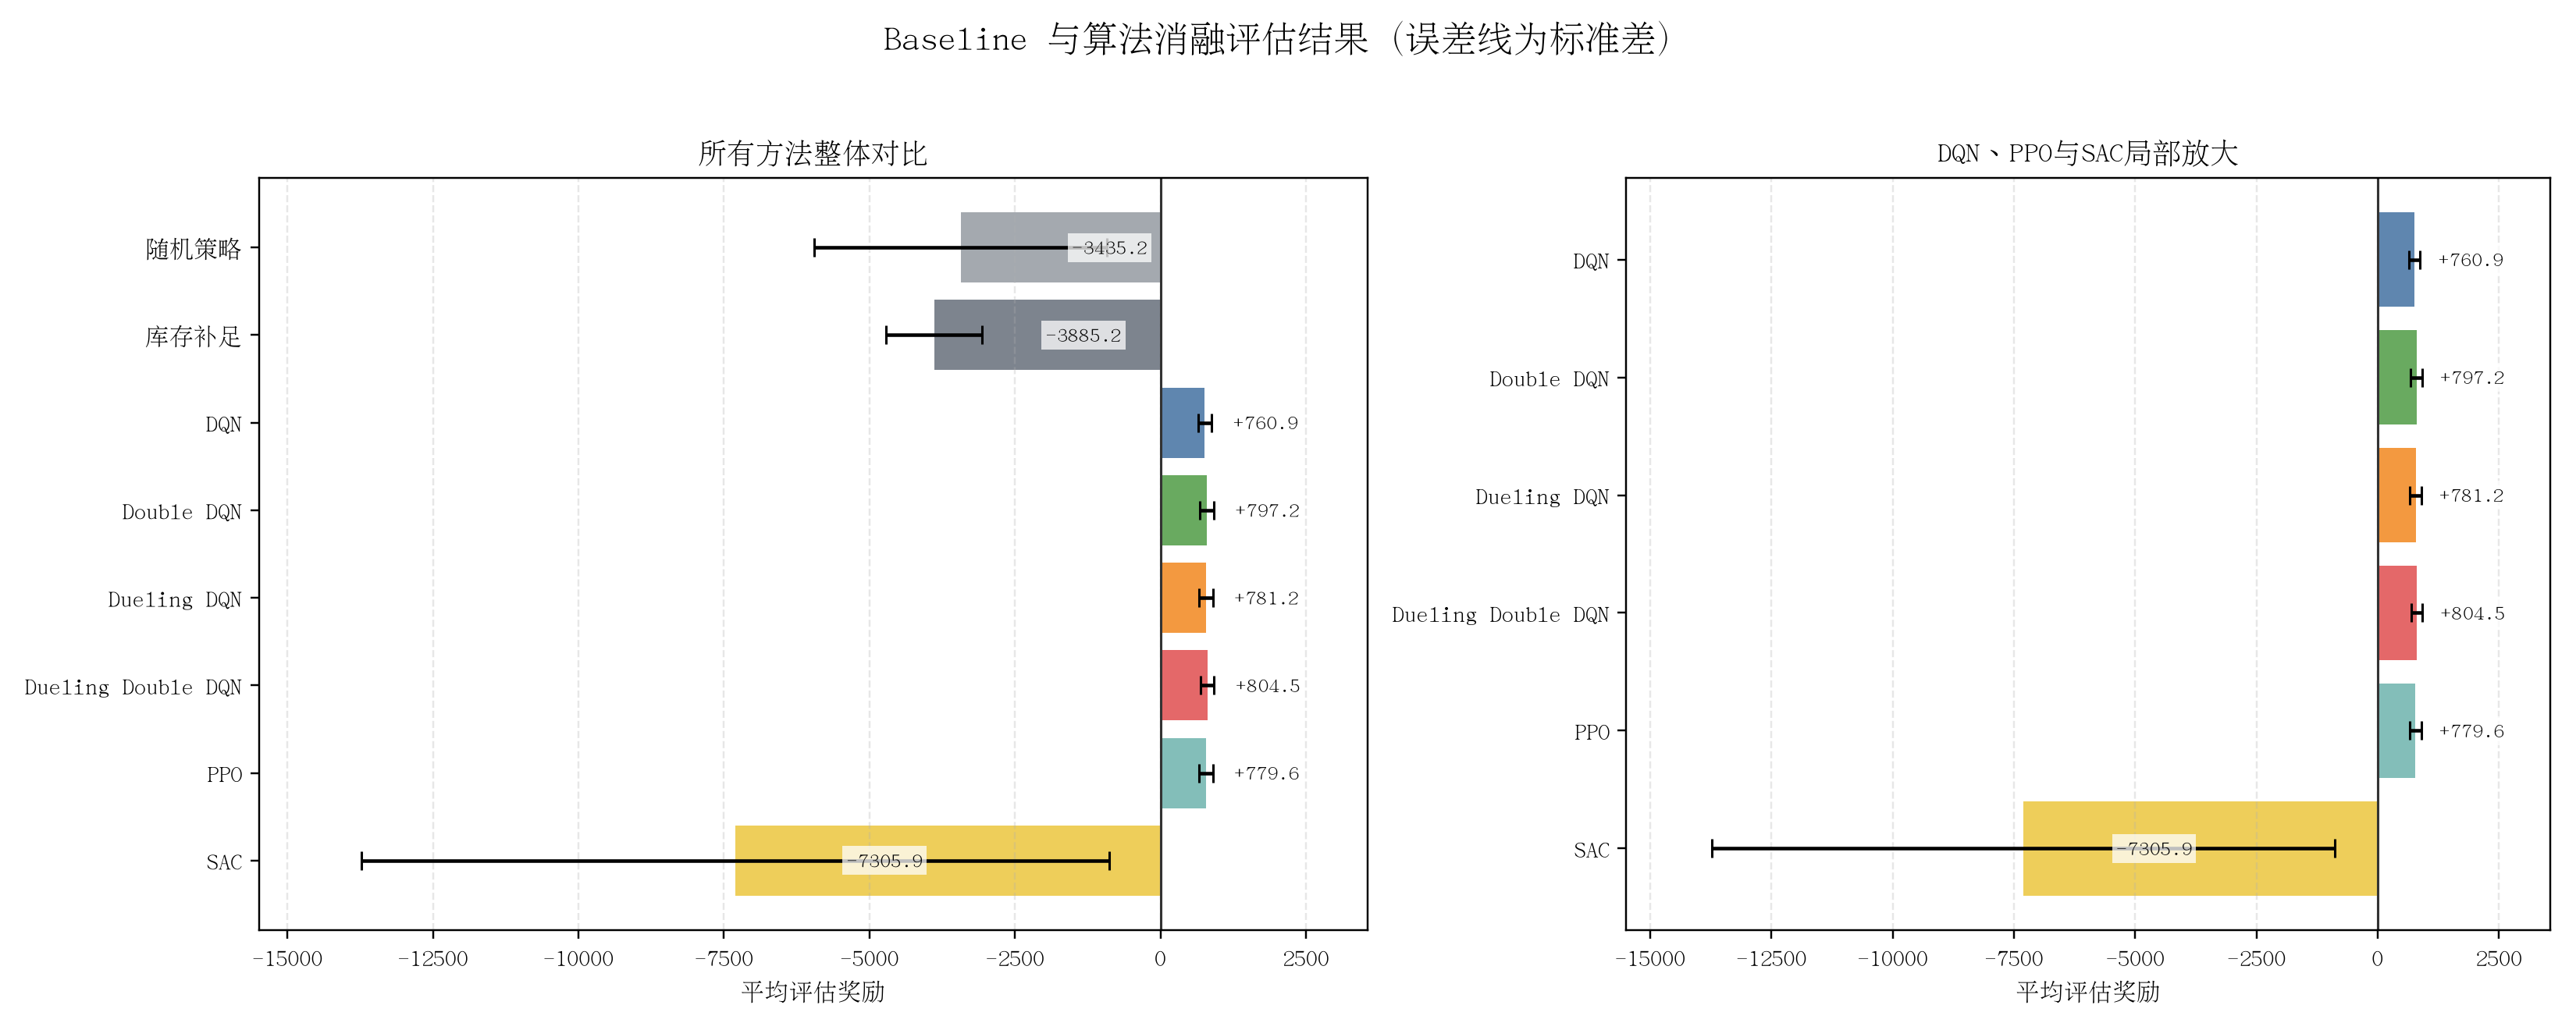
\includegraphics[width=0.9\textwidth]{../figures/baselines/baseline_comparison.png}
  \caption{各算法 3-seed 平均奖励对比（含标准差）}
  \label{fig:baseline-comparison}
\end{figure}

\subsection{结果分析}

\begin{itemize}[leftmargin=2em]
  \item \textbf{DQN 系列}表现最为稳定。Dueling Double DQN 以 804.46 的平均奖励位列第一，说明在网络结构与学习目标上的改进对抑制 Q 值高估有效。
  \item \textbf{PPO}在改进后平均奖励达到 779.59，部分 seed 达到 800 以上，但在 seed 42 上仅 753.50，仍存在一定方差。相比最初实现（seed 123 崩溃至 76.15），KL early stopping、reward scaling 与 best checkpoint 显著提升了稳定性。
  \item \textbf{SAC}在本任务上极不稳定，仅 seed 456 收敛至正值，其余两个 seed 因离散动作与奖励尺度不匹配导致策略崩溃。
  \item 规则策略 random 与 base\_stock 均为负奖励，远低于学习算法，说明学习环境中的局部优化空间较大。
\end{itemize}

\subsection{训练曲线}

图 \ref{fig:ddqn-training} 与图 \ref{fig:ppo-training} 分别展示了 Dueling Double DQN 与改进后 PPO 的训练曲线（含 3-seed 均值与标准差带）。

\begin{figure}[htbp]
  \centering
  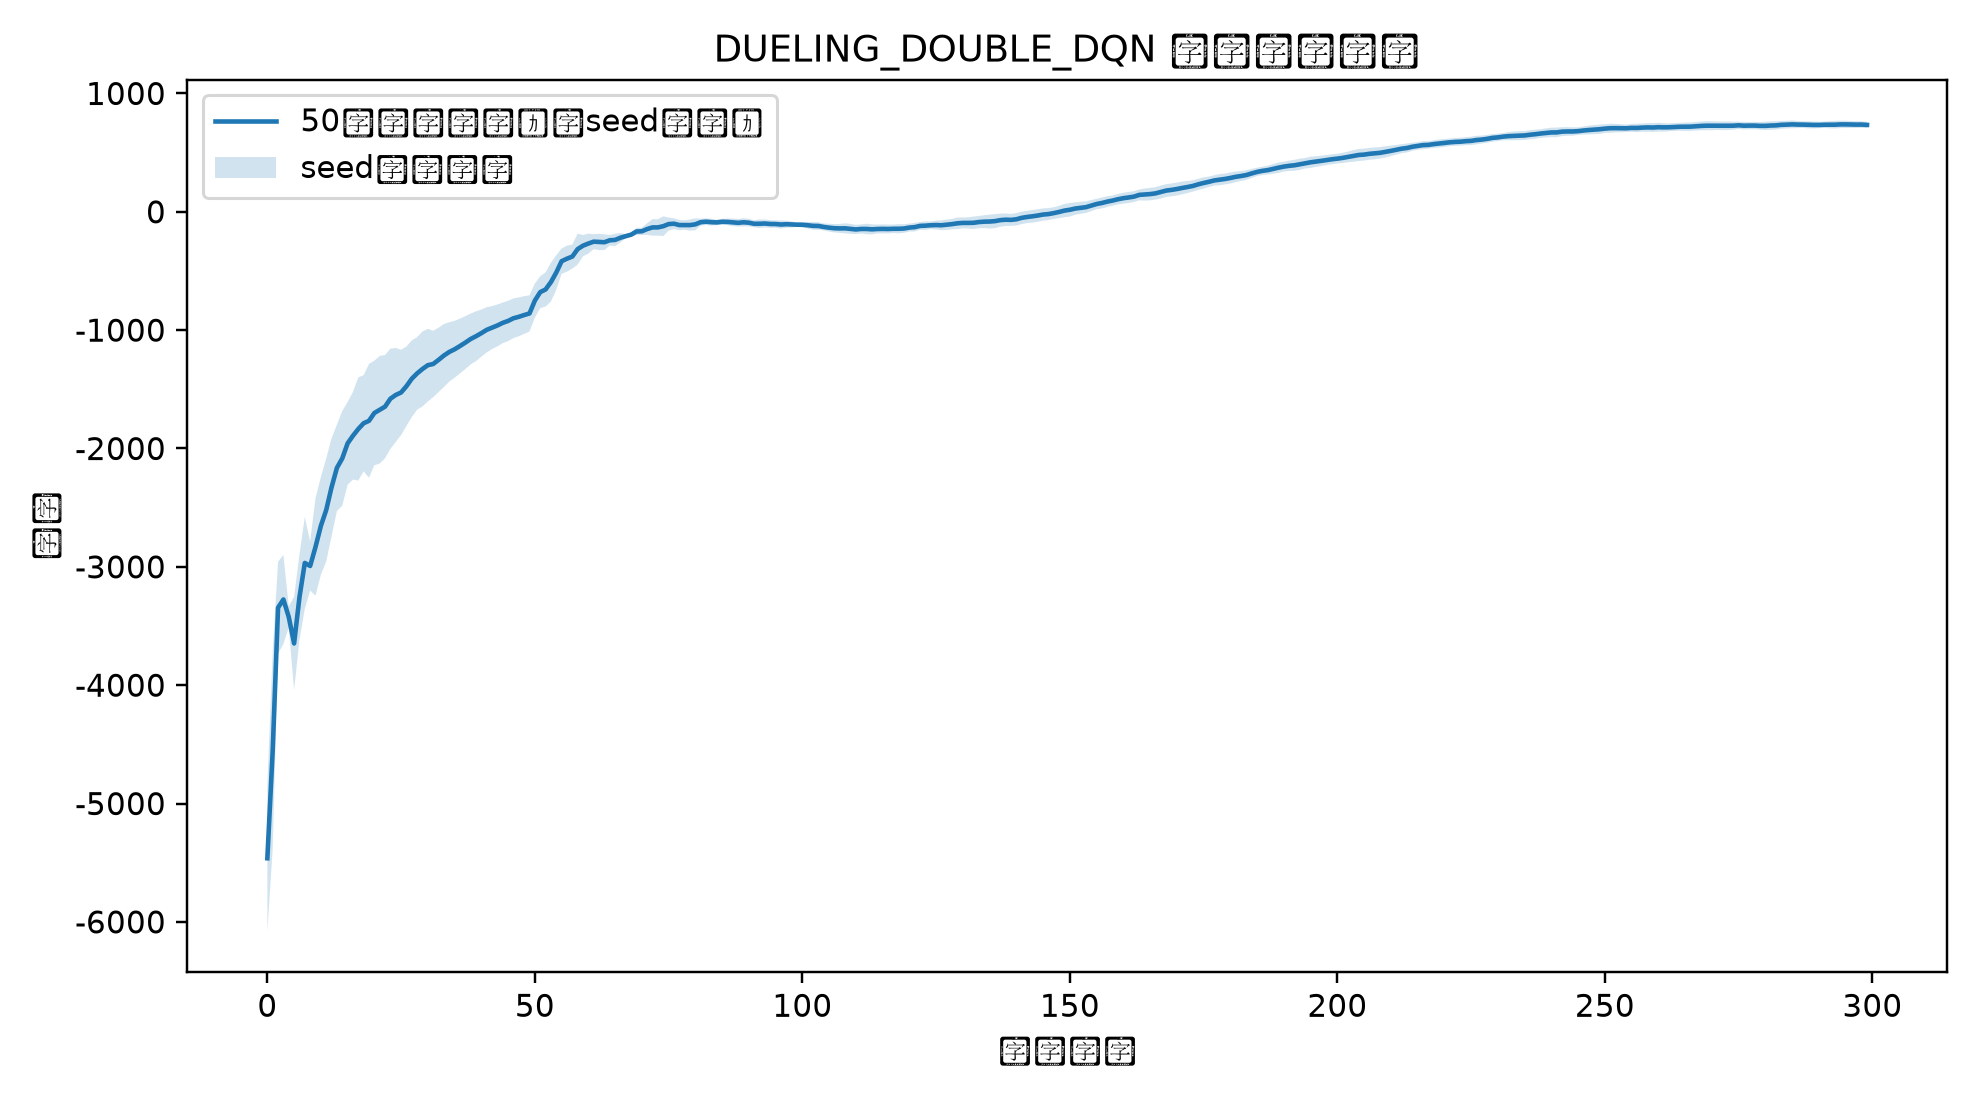
\includegraphics[width=0.85\textwidth]{../figures/baselines/dueling_double_dqn_training_rewards.png}
  \caption{Dueling Double DQN 训练曲线}
  \label{fig:ddqn-training}
\end{figure}

\begin{figure}[htbp]
  \centering
  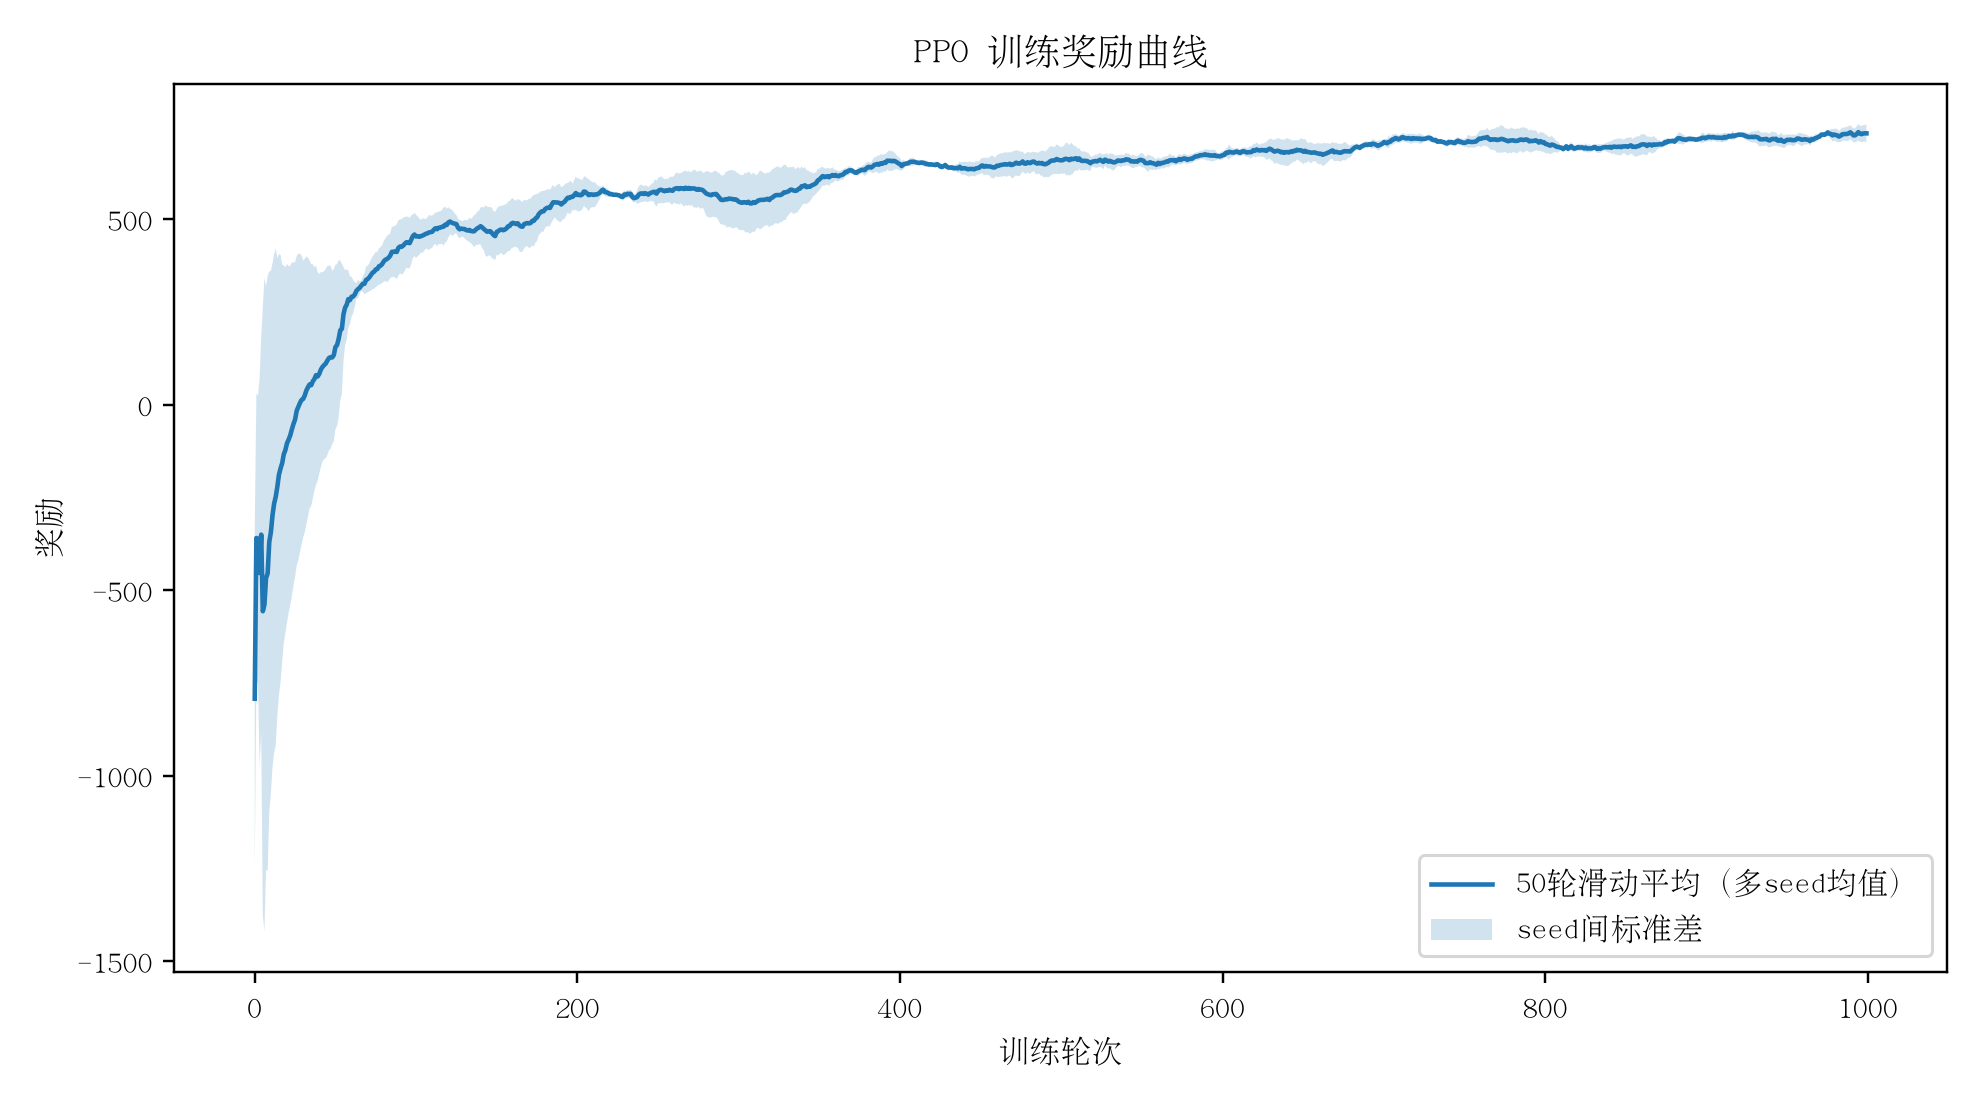
\includegraphics[width=0.85\textwidth]{../figures/baselines/ppo_training_rewards.png}
  \caption{改进后 PPO 训练曲线}
  \label{fig:ppo-training}
\end{figure}

\subsection{策略行为对比}

通过固定 seed 运行一个 episode，可对比不同策略的订货量、库存与即时奖励。Dueling Double DQN 学会了在需求波动时保持相对平稳的订货策略，而 PPO 在某些 seed 下仍存在订货量震荡，这可能是其方差较大的原因。

\begin{figure}[htbp]
  \centering
  \includegraphics[width=0.9\textwidth]{../figures/policy_behavior/behavior_comparison.png}
  \caption{最终策略订购行为对比}
  \label{fig:behavior}
\end{figure}

\subsection{背景策略与多智能体扩展}

表 \ref{tab:background} 比较了在其他企业采用 random 与 base\_stock 背景下的 Dueling Double DQN 表现。两者均值接近，但 base\_stock 背景标准差更低，说明规则化上下游可降低评估波动。

\begin{table}[htbp]
  \centering
  \caption{不同背景策略下的 Dueling Double DQN（seed=42）}
  \label{tab:background}
  \begin{tabular}{lcc}
    \toprule
    背景策略 & 平均 reward & 标准差 \\
    \midrule
    random background & 831.95 & 104.36 \\
    base\_stock background & 824.00 & 73.38 \\
    \bottomrule
  \end{tabular}
\end{table}

表 \ref{tab:multiagent} 给出了多智能体实验结果。独立训练三个 Dueling Double DQN 后，全链路 total reward 从负值提升至 3426.55，显著高于单智能体只优化企业 1 的情景（$-4663.73$）。

\begin{table}[htbp]
  \centering
  \caption{多智能体实验结果（seed=42，20 episode）}
  \label{tab:multiagent}
  \begin{tabular}{lcccc}
    \toprule
    方法 & 企业0 & 企业1 & 企业2 & 全链路 total \\
    \midrule
    random\_all & $-3763.38$ & $-4023.73$ & 3957.10 & $-3830.00$ \\
    base\_stock\_all & $-3509.93$ & $-3521.32$ & 3414.05 & $-3617.20$ \\
    single\_agent\_ddqn & $-3057.18$ & 831.95 & $-2438.50$ & $-4663.73$ \\
    multiagent\_ddqn & 468.77 & 538.60 & 2419.18 & \textbf{3426.55} \\
    \bottomrule
  \end{tabular}
\end{table}

\section{核心代码说明}

PPO 的 KL early stopping 实现如下：

\begin{lstlisting}
if self.target_kl is not None:
    with torch.no_grad():
        _, new_log_probs, _ = self.net.evaluate(
            states, actions,
            critic_states if critic_states is not None else None)
        kl = (old_log_probs - new_log_probs).mean().item()
    if kl > self.target_kl:
        break
\end{lstlisting}

Best-checkpoint 训练流程会周期性评估当前策略，保存并恢复最优模型：

\begin{lstlisting}
if eval_mean > best_eval:
    best_eval = eval_mean
    agent.save(best_path)
# 训练结束后
if best_path.exists():
    agent.load(best_path)
\end{lstlisting}

Centralized critic 通过将全局状态拼接后输入 critic\_body，使 value 估计能够利用其他企业的信息，而 actor 仍基于局部观测决策。

\section{讨论与未来工作}

\subsection{PPO 尚未稳定超过 DQN 的可能原因}

\begin{enumerate}[label=(\arabic*)]
  \item \textbf{样本效率}：DQN 通过经验回放重复使用样本，300 episode 即可获得稳定策略；PPO 的 on-policy 特性导致 1000 episode 的有效样本利用率仍较低。
  \item \textbf{离散动作与策略梯度}：动作空间小且订货量为整数，策略网络的 logits 容易过早坍缩到确定性动作，熵衰减后探索不足。
  \item \textbf{奖励稀疏与尺度}：单步奖励波动大，虽然已进行 reward scaling，但不同 seed 下优势估计方差仍可能过大。
  \item \textbf{背景策略随机性}：上下游为 random 时，环境动态高度非平稳，策略梯度方法对分布漂移更敏感。
\end{enumerate}

\subsection{后续方向}

\begin{itemize}[leftmargin=2em]
  \item 引入离线策略技巧（如 PPO with replay buffer / AWAC）提升 PPO 样本效率。
  \item 对 PPO 实施课程学习或预训练初始化，先用 base\_stock 背景预训练，再迁移到 random 背景。
  \item 将 PPO 扩展为 multi-agent（IPPO/MAPPO），利用 centralized training with decentralized execution 进一步降低方差。
  \item 尝试更激进的状态增强（需求历史、在途库存）以帮助策略网络更好地估计未来到货。
\end{itemize}

\section{结论}

本研究在啤酒游戏三阶供应链环境中复现并改进了 DQN、PPO 与 SAC 算法。实验表明，Dueling Double DQN 是当前任务上最稳健的高性能基线，平均奖励达 804.46。通过 GAE、reward scaling、KL early stopping、best checkpoint 与 centralized critic 等改进，PPO 的稳定性显著提升，平均奖励达到 779.59，部分 seed 超过 800，但尚未在所有 seed 上稳定超过 DQN。未来可通过提升样本效率、课程学习与多智能体训练进一步缩小并超越该差距。

\bibliography{refs}

\end{document}
